\documentclass{ltjsbook}
\usepackage{docmute} 
\usepackage{../../myStyle} 

\begin{document}
\VerbatimFootnotes
\chapter{いんたーみっしょん；Stanの概略と環境の準備について}
\label{PrepareStan}

このセクションでは，確率的プログラミング言語Stanを導入するにあたっての，周辺知識を解説します。授業中に解説するものではありませんし，ここに書かれていることのすべてを理解していないとStanを使えないというわけではありませんが，導入や利用にはトラブルやエラーも多く，その際に前提知識，周辺知識があるとないとでは理解度が大きく異なります。「わからなくても，なんとなく動いた」という状態で受講し続けるのは自身のためにならないだけでなく，\textbf{面白くない}です。知識があってはじめて価値がわかるということもありますので，共用としてご一読いただければと思います。

\section{はじめに}
この授業では統計言語としてのR，それを使う統合開発環境としてのRStudio，そして\keyterm{確率的プログラミング言語}{かくりつてきぷろぐらみんぐげんご}{stocastic programming language}としてのStanを利用します。大学でのPCルームの利用にはこれらの環境がすでにある程度準備されていますが，最新バージョンではありませんので，自分のPCに環境を準備することを強く推奨します。今後の研究室配属やその後の卒業研究などでも活用することになると思いますので，まずは自身のPC環境に準備することを考えてみてください。

この付録資料は，これらの環境を準備する方法について解説するものですが，提供されるソフトウェアのバージョンや対応する環境などは日々発展するものですので，必ずしも最適な情報提供になり得ません。基本的な情報は提供いたしますが，執筆時\footnote{この記事は2022年11月10日に加筆修正されました。}での情報であることも多く，より新しい情報についてはインターネットなどでキーワード検索を行なって，より良いものを探してみてください。

PCの操作が苦手に思っている人のために付言しますが，うまくいかなかったからといって癇癪を起こしたり，諦めたりしてはいけません。相手は機械ですから，命じられたことを愚直に実行しているだけです。また文房具のようなものですから，恐れて嫌うのではなく，愛して可愛がってあげることが肝要です。もしみなさんの中に，お持ちのPCに名前をつけていない人がいるようでしたら，今すぐ命名することをオススメします。パソコンが，と思うと腹が立ちますが，わたしのXXXちゃんが，と思うとエラーも「ちょっとご機嫌斜めなのかしら」と受け入れやすくなります\footnote{ちなみに私が初めて手に入れたノートPCには「秀吉」という名前をつけました。Macに変わってからは代々数学者の名前をつけることにしています。私はいま，GaussちゃんやHermiteちゃんを持ち歩いています。}。

また，困った時は教員，TA，先輩などに相談することが重要ですが，その際には症状や経緯を正確に伝えることが必要です。ペットを病院に連れていくときに「何もしてないのに勝手に病気になった。治してほしい」といわれても獣医さんは困ると思います。\textbf{普段の様子や症状についての丁寧な報告}を心がけてください。とくにPCは機械ですので，何もしていないのに壊れるということはありません。自分が自覚していないことであっても，「なにかをした」から様子がおかしくなるのです。自分はそんな大それたことはしていない\footnote{たとえば計算途中だけど時間が来たので電源をオフにした，といったことでも，内部ファイルにアクセしているときの中断であれば，十分にPCを破壊することができます。}，と思っても必ず何かトリガーがあったはずなのです。どこをクリックしたか，どういうコマンドを入れたかという\textbf{履歴をしっかりと把握し，丁寧に報告する}ことを心がけてください。

\section{Stanの位置付け}

\keyterm{確率的プログラミング言語}{かくりつてきぷろぐらみんぐげんご}{stocastic programming language}とは，確率モデルを記述し，データと合わせることで統計的推論をしてくれるコンピュータ言語のことです。Stanができる前は，\keytermL{BUGS}{BUGS}や\keyterm{JAGS}{JAGS}というものがありましたが，BUGsは開発が終わってしまいました\footnote{JAGSはまだ開発が続いているようで，Rから使うこともできます。}。今，こうした言語はStanが最先端だといって間違い無いでしょう。これらの言語は，具体的には確率モデルとデータの関係を記述することで，事後分布からの乱数を生成するというものです。以下ではこの言語の利用形式について解説します。

\subsection{コンパイラとインタプリタ}

プログラミングはコンピュータを動かすための仕様書を書くことです。ここで「コンピュータ」というのは計算機という意味だと思ってください。もちろんコンピュータは数字の計算だけでなく，音楽を奏でたりゲームを楽しませてくれたり，と色々なことができるのですが，その背後にあるのはとにかく0/1の数値演算です。0か1かという数字がどうして映像や音声，通信になるのか，と疑ってしまうほど異なっているようですが，それでもすべて数字の計算から構成されています。

コンピュータができ始めたごく初期の頃は，これを動かすのに0と1からなる数字の羅列で仕様書を用意していました。流石にそれではわかりにくく表現力にも乏しいので，次にできたのがマシン語とよばれる16進数による表現でした。この段階でも，知らない人にとっては暗号か，意味のある連なりに思えない文字列にすぎません。画面に線を引いて欲しい時に\texttt{line}という命令で伝えられるようになって，やっと普通の人間にも意味がわかるレベルになってきます。このように，人間がわかるレベルでコンピュータに命令が伝えられるような言語のことを\keytermL{高級言語}{こうきゅうげんご}と言います。高級言語は人間寄りで，直接コンピュータが理解できませんので，この高級言語を機械の言葉に翻訳するためのアプリケーションを介在させます。それがいわゆる\keyterm{プログラミング言語}{ぷろぐらみんぐげんご}{programming language}と呼ばれるものです。

プログラミング言語は，古くはBASIC，PASCAL，FORTANなどと呼ばれる書式のものがあり，その後出てきたC言語，その改良版であるC++言語\footnote{この\verb|++|という書き方は，C言語特有の「変数に1加える」という表記法であり，C言語の改良版という意味でC++と命名されています。読み方はシープラスプラスですが，シィプラプラの愛称でも知られています。}などが有名です。他にもJAVAやObject C，Pythonなどが有名ですね。Rも言語の一種で，統計解析に特化したものです。また，この授業で扱うStanという\keyterm{確率的プログラミング言語}{かくりつてきぷろぐらみんぐげんご}{stocastic programming language}は，確率モデルの分析に特化したものです。みなさんがデータサイエンス業界に進むのであれば，PythonやRを使えるようになっておくといいでしょう。これらの言語の特徴の1つは，パッケージを追加することで機能が拡張できることにあります。とくに\keytermL{機械学習}{きかいがくしゅう}系(AIなど)のパッケージが豊富なのがPythonです。またこれらの言語は基本的にフリーソフトウェアであり，導入にお金がかからないところもポイントですね。タダで始められるおもちゃみたいなものです！\footnote{余談ですが，Scratchや任天堂Switchの「ナビつき! つくってわかる はじめてゲームプログラミング」などにみられる，GUIベースのプログラミング言語もあります。これはプログラミングの要素がアイコンやキャラクターになっていて，それらを組み合わせることで計算させるという方法をとっています。その操作のしやすさ(ミススペルがない！)から，小学生などにも導入できる素晴らしい取り組みです。同様の発想は，LOGO言語などにもみられました。}\footnote{PerlやJava Scriptなど，Webブラウザ上で動くプログラミング言語もありますが，これはブラウザ上での操作に限定されており，数値計算にはあまり向かないのでここには取り上げていません。さきほどあげたJAVAとJAVA Scriptは別物なので注意してください。}\footnote{GUIアプリケーションを作ることに特化した言語もあります。数値計算と違って，マウスがどこでクリックされたか，と言った「動き」を契機としてプログラムが走る，イベントドリブン型の言語で，Microsoft社のVsial Basicなどが有名です。これはMicrosoft Office製品の中に埋め込むこともでき(VBA)，これを使うとExcelでも高度な統計解析ができたりします。Excelを使った統計ソフトウェアとして代表的なものにHADがあります\textcite{HAD}。他にもDelphiなどの言語がありました。}\footnote{\textcite{Language2016}には，数え方にも癖がありますが，117ものプログラミング言語が紹介されています。}

プログラミング言語の分類には，その設計思想や書き方などを基準にすることもできますが，実行方法を基準にするものとして\keytermL{インタプリタ}{いんたぷりた}型と\keytermL{コンパイラ}{こんぱいら}型とに分けることができます。
インタプリタ型は，interpret，つまり翻訳型です。これは毎回の命令を機械語に翻訳して実行していきます。Rはインタプリタ型言語で，毎回の命令を逐一翻訳して実行していきます。Rを実行するとき，コンソールに\verb|>|というマークが出ていますよね。これはRが聞き耳を立てている状態，入力待ちの状態なのです。ここに命令を書くと(たとえば\verb|2+3|と書く)，Rはすぐさま答えを返してきます(たとえば\verb|[1] 5|と返す)。基本はこのように一問一答，ひとつひとつの命令を毎回機械語に翻訳して実行し，その答えを出力するという手続きをとっています。もちろん私たちの分析プログラムは，一行で書ける簡単なものではありませんから，複数行に渡る長々としたファイルを書くことが多いでしょう。こうしたファイルはプログラムともいわれますし，一行一行の命令のことを\keyterm{スクリプト}{すくりぷと}{script}ということもあります。プログラムファイルあるいはスクリプトファイルを開いて，一行ずつ実行するのがRの基本的なスタイルであり，RStudioはスクリプトファイルを編集する\keyterm{エディタ}{えでぃた}{editor}がセットになっているのが便利な点なのでした。

これに対して，インタプリタ型は，スクリプトファイルをまとめて機械語に翻訳(コンパイル)し，実行ファイルというのを別途作ります。その上で，実行ファイルを実行すると計算が進められるのです。どうしてこんな手間がかかることをするのでしょうか。ひとつには，ひとつひとつの命令分を逐一翻訳しているのでは，実行スピードが遅くなるということが挙げられます。命令を逐一聞き耳を立てて待ち，全ての命令を聞き終わるまで途中の指示を記憶しておいて，命令文が終わってはじめて行動に移す，というのでは記憶容量も時間もかかるわけですね。これに対して，一連の計算命令文書を一括で渡すことができれば，機械は内部的に効率よく計算手順を配置して実行できます。コンパイラ型は計算スピードが速いのです。ちなみに実行ファイルは機械がわかる言葉に書き換わっているので，人間が見ても意味がわかりません。また，OSやCPUに理解できる形に書き換えていますので，MacOSの実行ファイルをWindowsで実行する，ということはできません。翻訳後の言語が違うからです。スクリプトファイルは環境を超えて共有できますが，それを翻訳したり最適化したりする仕組みは，個別の環境に依存します\footnote{ちなみにRやRstudioはもちろん，WordやExcelなどのオフィスアプリ，果てはOSそのものも，コンパイルされた実行ファイルをPCが計算して実行しているに過ぎません。}。

Stanはコンパイラ型です。Stanのファイルを読み込んで，機械にわかるように「事後乱数生成命令文」に翻訳して実行します。確率モデルから乱数を生成するのは非常に高度な計算機能ですから，コンパイルしてまとめておくことでスピードアップの効率が断然良くなるわけです。コンパイラ型の利点はこのスピードにありますが，欠点は「命令に変更やミスがあれば翻訳し直さなければならない」というところです。あり得ない命令を出しているようであれば，コンパイルの段階で「おかしな文法だよ」とエラーを出して翻訳を止めてくれます。翻訳が通れば良いかというとそうではなく，翻訳はあくまでも文法上の手続きであって，数値や内容に間違いがあっても翻訳自体は完了させることができるのです。翻訳(コンパイル)には少し時間がかかりますから，文法上も内容上も間違いのない命令分をしっかり準備しておくことが重要になってきます。
\subsection{ファイルのやり取りについて}
ここで，R/RStudioをつかってStanを使う際の，ファイルのやり取りを見ておきましょう(図\ref{fig::pp_01})。

StanのコードはRのコードの中に書くこともできますが，別のファイルに保存しておくのがベターです。Stanファイルは拡張子を\verb|.stan|とすることが一般的です。このファイルの中身はプレーンテキストでコードを書いていますから，一般的なエディタ\footnote{エディタとはASCIIファイル，いわゆるプレーンテキストを編集するアプリケーションの総称で，OSにデフォルトで「メモ帳」などの名称で含まれています。デフォルトのアプリは文字を読み書きできるだけですので，もう少し発展的，あるいは便利な拡張機能を持っている専用のアプリを使うことが一般的です。筆者は最近もっぱらVS Codeというエディタを利用しています。他にもMacOSでしたら，「mi」というアプリを好んで使っていました。Windowsでしたら「秀丸」というアプリが有名です。Ubuntuにはgeditというアプリがデフォルトで入っていますし，歴史やユーザの多さではvimやemacsなどがあります。Linux界隈で，vim派かemacs派かの話題は，きのこたけのこ戦争ばりに激しい戦いになります。}で編集できます。RStudioのエディタ画面も必要十分なエディタ機能を持っていますので，RStudioをエディタとして利用するのがいいでしょう。

RStudioでFile > New Fileとして新しいファイルを開くときに，Stanファイルとして開くことが可能です。Stanファイルとして開くと，初心者向けの配慮からか，最初からちょっとしたコードがすでに書かれています。コードの書き方を示すサンプルコードなのですが，実際にこのコードを使って何かすることはありませんので，中身は全部削除してしまいましょう。それでもRStudioはその画面がStanファイルのものだということは認識していますから，そこで書いたファイルはStanファイルとして扱ってくれます。ここでまちがって新しくR Scriptで開いてしまった，というときに，保存するときだけ\verb|.stan|をつけておけばいいか，という対応をすると失敗します。RStudioでは拡張子をあえて表示していませんので，ファイル名として\verb|hoge.stan|と書くと実際には\verb|hoge.stan.R|というファイル名になっています。拡張子は最後のピリオドで判断されますので，これはRファイルなのです。このミスを防ぐために，ファイル名にピリオドは使わないこと，ファイルの種類を変える時はエディタ画面の右下でファイル種別を選択してください(図\ref{fig::pp_02})。

\begin{figure}[ht]
	\centering
	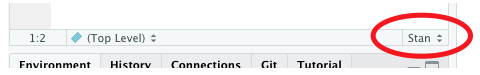
\includegraphics[keepaspectratio,width=0.8\linewidth]{../images/prepare/fileStyle.png}
	\caption{ファイル種別の変更}
	\label{fig::pp_02}
\end{figure}

RStudioを使ってStanを書くと便利なことがいくつかあります。ひとつは強調表示機能で，ブロックや関数名などStanで使うことが決まっている専門用語は色やフォントが変わって表示されます。\verb|transformed parameters|のように長い専門用語を書くときはミススペルが心配ですが，書いた後で強調されなければスペルミスがある，ということがわかります。もうひとつの利点は文法チェックの機能です。コンパイル型なので，Stanに書かれた命令文は実行前に一括で翻訳されますが，スペルミスや型の違いなど，文法的に間違っているところがあればこれも自動的にチェックして警告記号がでます。またStanファイルが開かれているペインの左上に\verb|Check|というボタンがあり，これを押すことでファイル全体の文法チェックをしてくれます。もし文法上の問題がなければ，「hogehoge.stan is syntactically correct.(hogehoge.stanというファイルは文法的には正しいですよ)」というメッセージがコンソールに表示されます。逆にいうと，これが表示されないというときは何か間違っているので，コンパイルに進む前に修正しましょう。

さてこのようにしてStanファイルを準備します。また分析用のデータセットが外部ファイルにある場合などは，これまで同様，当該プロジェクトフォルダ内に置いておくと良いでしょう。これらはいずれも，Rのコードで呼び出して使うことになります(図\ref{fig::pp_01}の1.と2.のステップ)。Rでは，Stanファイルやデータファイルを読み込んで，これをPC内部にあるStanに渡します(図\ref{fig::pp_01}の3.のステップ)。StanはRと違う言語であり，Stan独自の計算機能で計算してくれるわけですから，RとStanの橋渡しが必要になります。Rではこれを\verb|cmdstanr| や\verb|rstan|というパッケージを経由して行います。これらのパッケージがStanを呼び出してくれるわけです\footnote{このように，Stanは独立した計算環境であり，R以外のアプリケーションから呼び出して使うことが可能です。Pythonから使いたい場合は，PyStanというパッケージ経由で，Juliaから使いたい場合はStanJl，コマンドラインから使いたい場合はcmdstanといったように，いろいろなルートがあります。}。

データと確率モデルの関係を記したStanファイルと，データのそのものを受け取ったStanは，コンパイルしてPC内に乱数発生装置を作ります(図\ref{fig::pp_01}の4.のステップ)。事後分布の関数を書き出すのではなく，その形状とそれを代表する乱数を作る状態をもつわけです。Rの指示をうけて，そこから必要な数だけ乱数を作り出します(図\ref{fig::pp_01}の5.のステップ) 。Rはこれを受け取って，統計解析を始めるわけです。Rは統計に特化した言語ですから，集計や可視化などの作業はお手のもの。事後分布から得られた大量の乱数は，事後分布の特徴を反映した大量のデータセット，事後分布の具体例たちになっているのでした。

分析の進め方は以上のようになります。Rでデータを整形し，Stanのファイルも別途用意して，RからStanを呼び出す，Stanか返してきたデータをRで解析する，ということです。Rの拡張子は\verb|.R|で，Stanの拡張子は\verb|.stan|，データファイルの拡張子は\verb|.csv|などでしょうか。いずれにせよ，複数の種類のファイルをやり取りしながら進めるので，相互の関係についてしっかり理解しておく必要があります。


\begin{figure}[ht]
	\centering
	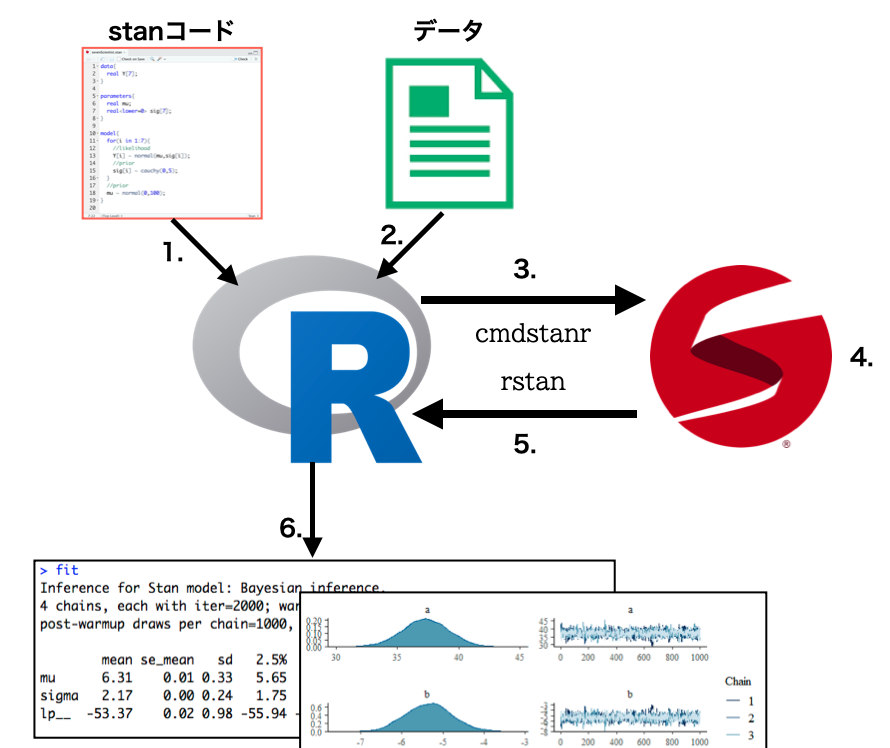
\includegraphics[keepaspectratio,width=0.8\linewidth]{../images/prepare/R_stan.png}
	\caption{R/RStudioとStanファイルのやり取り}
	\label{fig::pp_01}
\end{figure}
\subsection{2つのルート}
ここではRからStanを呼び出す2つのルート，具体的には\verb|rstan|パッケージと\verb|cmdstanr|パッケージについて説明します。
この2つのパッケージは，いずれもStanを呼び出してつかう，RとStanの間を取り持つインターフェイスの役割を持ったパッケージです。間を取り持つだけなので，Stanファイル自体は同じであっても構いません。同じStanファイルを\verb|rstan|から呼んでも，\verb|cmdstanr|から呼んでも，結果は同じです。ただしインターフェイスが違うので，結果の扱い方が変わってきます。他にも違うところがいくつかありますので順に説明していきますが，結論からいうとこれから\footnote{執筆時点，2022-11-14現在}は\verb|cmdstanr|のほうを使うほうがお勧めです。

歴史的には\verb|rstan|のほうが古くから存在します。このパッケージも最初の頃は導入に一苦労するものでしたが，2016年ごろからCRANを通じて配布されるようになりました。要するに，他のパッケージと同じように，\verb|install.packages("rstan")|とRで書くだけで導入できるようになったのです。このようにして導入するとわかりますが，\verb|rstan|は多くの依存パッケージがあります。StanはコンパイルするのにOSに応じたC++コンパイラを借用しますが，RからC++を呼び出すパッケージやRとC++の間に入るStanHeaderと呼ばれる緩衝材など，関連する多くの環境を整えてやっとRからStanへのルートが通じるのです。ユーザにとってはそのような苦労は知ったことではない，という感じですが，「間に多くの調整が入る」ということがエラーの温床になっていました。つまり，いくつかの内部的ステップのどこかでバグがある，互換性がない，というようなことがあると，Stanファイルが同じでも，バージョンが変わるとコンパイルできないということがよくあったのです。Stan本体の方も開発が盛んですから，Stanの新しいバージョン，新しい機能を使いたいと思っても，パッケージが対応するのを待たなければなりません。パッケージが対応しても，途中の媒介パッケージが追いついていなければバグになったりします。これらを使うRやOSもアップデートしていきますから，その度に「動かなくなる」ということはよくありました。研究の再現性が問題になる昨今ですが，自分の研究とデータであっても，自分の環境で再現できないということが少なくなかったわけです\footnote{実際RやOSのアップデートに関わるエラーは大変で，筆者は一度OSをアップデートした後半年ほどStanが使える環境が作れず，研究が頓挫したことがあります。そのために別途，PCを購入し直したぐらいです。}。そうなると，今動いているからそれでいい，と環境のアップデートを控えるようになりますが，ご存知の通りOSやアプリのアップデートはバグやセキュリティホールの修正など，安全につかうための基本的な機能に関わってきますから放置もできない，という問題があるわけです\footnote{OSのアップデートなど，通知が来ても「今支えているからいいや」と無視する人もいますが，できればOSやアプリは最新版であるほうが良いのです。セキュリティホールの問題などを放置しておくと，インターネットを介して自分のPCの中身が全部見られて公開される危険性があります。Stanしか使わないネットに繋がないPCというのがあればいいのかもしれませんが，文房具としてのPCはもっと一般的な用途がありますから，そうもいってられませんよね。また，一昔前のOSアップデートは，アップデートの失敗でPCが動かなくなるというようなこともありましたから，アップデートが公開されてすぐに対応するのは「人柱」などと揶揄されていましたが，最近はそういったこともほとんどありませんので，安心して常に最新の状態にしておいてください。}。

このような不安定な環境になる原因は，RとStanの間にあるさまざまな障壁と，それをなんとかして調整しようという媒介パッケージの存在でした。そこでなるべくシンプルにRとStanをやりとりする方法はないものか，ということで考えられたのが\verb|cmdstanr|です。これはコマンドライン\footnote{MacOSやLinuxでは端末，ターミナル，Windowsではコマンドプロンプトなどと呼ばれる，PCに直接コマンドで命令を出すプリミティブな実行環境です。}からStanを呼び出す\verb|cmdstan|をRから呼び出して使おう，というものです。StanをRになんとか取り込んで動かす，というのではなく，Stanの部分はOSのプリミティブな環境にお任せ，Rは結果をもらうだけ，というシンプルな設計にしようというわけです。たとえば\verb|rstan|はStanの計算結果をRオブジェクトとして取り込みますが，\verb|cmdstanr|は実はMCMCの結果はcsvファイルのような形で吐き出しており，それを読み込んで使います。御用聞きや仲介業者を介して情報をもらうのではなく，現地で直接買い付けしてくるようなイメージでしょうか。このように間に挟むものを減らすことによって，不安定な要素をなくしたわけです。

\verb|cmdstanr|はStanとRの複雑な絡まりを排していますので，Stanの開発が進めばすぐにそれをRに届けることができます。たとえば2022/11/14現在で，公式にリリースされている\verb|rstan|のバージョンは2.21.1ですが，\verb|cmdstanr|が呼び出すstanのバージョンは2.30.1です。\verb|cmdstanr|のほうが新しいものに対応できていますね。このように，\verb|cmdstanr|がでてきてからはこちらの対応，反応が早く，また動作も安定的ですから，よりお勧めしやすくなっています。

これまでに出ているRでStanを使う方法を解説したテキストの多くは，\verb|rstan|をつかっていますので，今それを使うためには多少の読み替えが必要です。とはいえ，Stanのコード自体はそのまま使えるものがほとんどで，Rとのインターフェイス，やりとりの方法が違っているだけです。\verb|cmdstanr|には，結果を\verb|rstan|で得られたオブジェクトに変換する関数も含まれていますから，これらを使って変換すれば，以後のコードは\verb|rstan|準拠のものでもエラーになることはありません。このテキストでは第2版から\verb|cmdstanr|を中心にするように切り替えましたが，以前のコードでも本質的に問題はありません。

\section{導入の概略}
環境の導入は，OSの種類によって変わります。WidowsなのかMacなのか，あるいはLinuxなのかといった違いに合わせて導入を考えてください。
OSの種類で言えば，Linuxは全体的にCUI操作が主であり，堅牢かつ合理的な使い方ができるものです。如何せんマイノリティですので，ググってもあまり情報が出てこないところが玉に瑕です。
MacはLinuxベースのOSになっているので，比較的堅牢かつ合理的な使い方ができます。ハードウェアもOSも1つの会社(Apple)が作っているので，サポートもしやすいという利点がありますが，日本では少数派なのが残念なところです。
Windowsは多数派のOSですが，OSメーカはソフトウェア会社でハードウェアが別会社なことが多く，利用される範囲は広いのですが，その分問題が生じたときにケースバイケースになりがちです。多くのハードウェアの違いを吸収するために最大公約数的な設計をするせいか，ソフトウェアデザインの統一性がないところが欠点です。ユーザ数は最も多いので，一生懸命調べたら同じような問題で困っている同じような機体の人に出会える可能性が高いのがせめてもの救いです。また光明としてWindowsOSもLinuxベースの仕組みを取り入れ始め(WLS)，比較的合理的な振る舞いができるようになったことが挙げられますが，OSのグレードによって導入のしやすさが異なります。

ちなみにChromeOSやiOS, Androidなどタブレット・スマートフォンでの統計環境の利用は限界があります。これらは計算結果を利用するフロントエンドとしては非常に高機能なのですが，インタラクティブに使うことには不向きです。いわば書籍のように多くの情報を一方的に与えてはくれるのですが，ユーザが計算するといった働きかけの補助になるような(ノートとペンのような)使い方ができませんので注意してください。

さて，環境の導入として2つのルートを紹介しましょう。第一のものが最も基本的なアプローチで，自分の手元の環境を作り上げるというものです。これを\textbf{ローカル環境}での構築と呼びます。ローカル環境は自分だけの環境ということなので，自分の責任でもってしっかりと環境構築をできます。第二のアプローチとして，ある程度できあがった環境を丸ごと取り込む，\textbf{仮想環境}での構築という方法があります。PCのOSの中に別のマシン・別のOSをさらに憑依させて使うようなやりかたで，これができると取り込む環境は完成しているので細かい設定をする必要がありません。問題は「憑依させる」準備がいろいろ大変であるということです。また憑依させたPCはブラウザ経由でアクセスすることになることにも注意してください。
% 最後の方法は，\textbf{サーバの利用}です。これは環境を構築するのではなく，すでに誰かがどこかで構築してくれたサービスを受け取るという，受動的な方法です。サービスを受け取ることのメリットは作り手の苦労を知る必要がないことですが，サービスが打ち切られると手元に何も残らなくなるという問題があります。この講義の受講者は，第一，第二の方法でどうしてもうまくいかなかった場合に，私の方からサーバ環境によるサービスを提供しますので，最後の砦だと思っておいてください\footnote{ケチくさいこと言わずに全員に提供しろよー，と思うかもしれませんが，サーバが貧弱で全受講生が一斉にアクセスするとサーバが止まってしまう可能性が高いからです。ちなみにサーバを強くするためにはたくさんのお金がかかりますので，私個人のサービスでは限界があるのです。}。

\subsection{導入方法1；ローカル環境での構築}

ローカル環境での構築は，R，RStudioの導入から入ります。ここは既にできている人もいるかもしれませんが，念のためバージョンが最新のものかどうかを確かめておいてください。
ローカル環境構築の方法がわからない人は，「RStudio」「インストール」などのキーワードでウェブ検索し，自分の環境にあった例を見つけてそれをみながら進めると良いでしょう。
参考までにいくつかあげておきますと，新しいものでは，高知工科大学柳井先生のこちら\url{http://yukiyanai.github.io/jp/resources/}とか，Quiitaの記事\url{https://qiita.com/hujuu/items/ddd66ae8e6f3f989f2c0}が良いでしょう。
書籍では，手前味噌で恐縮ですが\textcite{kosugi2019}などが良いでしょう\footnote{インストールに際しては，RStudio DesktopのFree editionを選んでください。RStudio CloudやRStudio Serverは別のものです。}。

次に確率的プログラミング言語，Stanの導入を行います。StanをRから使うためのパッケージとして\texttt{cmdstanr}と\texttt{rstan}という2種類があるという話はしました。かつては\texttt{rstan}のほうがよく使われていたのですが，最近は\texttt{cmdstanr}のほうが安定的に動作し，開発も盛んになっているので，2022年度後期からは\texttt{cmdstanr}をこの授業のデフォルトパッケージとしたいと思います。このパッケージの導入には，公式サイト\url{https://mc-stan.org/cmdstanr/articles/cmdstanr.html}を参考にしましょう。「cmdstanr インストール」で検索すると色々な紹介サイトが出てきますので，自分と同じ環境でなるべく日付の新しいものから参考にしていくといいでしょう。

インストールにあたっては，Stanがコンパイルされるときに利用するC++言語環境が必要です。これはMacOSであればXcodeの導入が，WindowsであればRtoolsでの導入が必要になります。
\paragraph*{MacOSユーザの場合}AppStoreでXcodeと検索し，XcodeをインストールすればOKです。

\paragraph*{Windowsユーザの場合}RtoolsというR周辺のツールをインストールする必要があります。\url{https://cran.r-project.org/bin/windows/Rtools/}にいって，自分のRのバージョンにあったRToolsをインストールしてください。
この他にもWindowsユーザは導入にあたって色々障壁にあたることがありますので，こちらのサイト\url{https://norimune.net/3609}なども参考にしてみてください。
% 2022-09-18 17:35:05 rstanを第二候補に
% StanをRから使えるようにするものとして，\texttt{rstan}パッケージがあります。
% これもOSごとに導入の方法が違いますので，公式サイト\url{https://github.com/stan-dev/rstan/wiki/RStan-Getting-Started-(Japanese)}をみて導入にチャレンジしましょう。このサイトは「rstan getting started japanese」などで検索すると見つけることができます。

\subsection{導入方法2；仮想環境での構築}

第二のルート，仮想環境を構築する場合ですが，これについては我らが国里先生が大変詳しいサイトを作ってくださっています。
日本心理学会のチュートリアルワークショップ，「再現可能な日本語論文執筆入門：jpaRmdで実現する再現可能で低コストな日本語論文執筆のはじめの一歩」で使われた時の資料集がそれで，このサイト\url{https://ykunisato.github.io/jpa2021-tws-jpaRmd/}の事前準備編をよく読むと導入できます。通信環境にもよりますが，慣れているとものの10数秒でシステム導入できるという優れものです。面倒な設定が怖い人は，是非試してみてください。


\section{導入方法3；外部サーバの利用}

最近，Google社がオンラインで利用できる分析環境，Google Colaboratoryを提供してくれています。
これはGoogle社が提供する，ブラウザで実行できるプログラミング環境です。Googleが教育，研究用に提供しているもので，90分間は無料で利用できます。90分を超える場合でも，書いたプログラムを保存しておけば，新しいセッションを開始することで続けて利用できます。これを用いる利点は，どのユーザにも同じ環境を提供できることです。

基本言語環境はPythonで提供されており，Jupyter Notebookを使いますが，次のアドレス(に含まれるコード)を使えば言語環境をRに変えて利用することができます。
\begin{center}
	\url{https://colab.research.google.com/notebook#create=true&language=r}
\end{center}

ここでウィンドウにRのコードを入力し，実行していきます。\texttt{cmdstanr}や\texttt{rstan}もインストールできます。
インストールに際して，\verb|install.packages("rstan")|のように入力することもできますが，この方法ですとインストールに随分と時間がかかります。
そこで少し例外的ですが，システムコマンドを直接利用して，\verb|system("apt install -y r-cran-rstan")|のようにすることで，大幅にスピードを短縮することができます。

\subsection{導入後の確認}
インストールが終わったらサンプルコードを実行して「動くかどうか」を確かめてみてください。サンプルコードはGetting started with CmdStanRのサイト，あるいはRStan Getting Startedのサイトに掲載されています。
どちらのパッケージから実行しても，文字列がズラズラっと出力されればとりあえず動いたと思っていただいて結構です。赤い文字やエラーなどが表示されうる，あるいは全く表示されない場合は，インストールがうまくいっていないことを疑いましょう。上に戻って，丁寧に説明に目を通して一歩ずつ進めてください。機械に命令することですので，自分勝手にショートカットしたり変更したりしないことが重要です。
\section{Stanを使ってみよう}
具体的なStanコードの書き方や統計モデルへの応用については，本書の次の章から順に説明していきます。
それに先立って，全体的な注意をしておきたいと思います。具体的には，バージョンによる違い，パッケージによる違い，そして本書の以下の章で使う関数の紹介です。

\subsection{バージョンによる書き方の違い}
\verb|cmdstanr|と\verb|rstan|はパッケージの使い方以上に，それらが呼び出すStanのバージョンの違いがあります。上で解説したように，\verb|cmdstanr|のほうが最近は開発が進んでいて，より新しいStanの機能を使っていることになります。
バージョンが違っても，基本的な書き方などに違いはないのですが，バージョン2.26からStanの文法に変更が予定され，導入されました。


データXがN人分あったとします。数学的フォームでは，$X_1,X_2,X_3,\cdots, X_N$というようなものですね。これはコンピュータ上では\verb|X|と名付けられた配列，サイズ$N$というように考えます。これは，Stanでは次のように書くものでした。
\begin{lstlisting}[language=C++,label={code:PRE_01},caption={Stan2.26以前の書き方}]
int n[5];
real a[3, 4];
real<lower=0> z[5, 4, 2];
vector[7] mu[3];
\end{lstlisting}

これらは上から順に，サイズ$5$の整数変数\verb|n|,サイズ$3 \times 4$の実数変数\verb|a|，下限$0$のサイズ$5\to,es4\times2$の配列\verb|z|，長さ$7$のベクトル\verb|mu|が3つ，ということを意味しています\footnote{ベクトルは数字をセット，人まとめとして演算するものです。最後の変数は，7つの数字のセットが3つという意味で，7つセットで1つのまとまりですよ，ということを明示的に宣言していることになります。}。

この書き方が，Stanのバージョン3.32以降は次のような書き方になります。
\begin{lstlisting}[language=C++,label={code:PRE_02},caption={Stan2.32以降の書き方}]
array[5] int n;
array[3, 4] real a;
array[5, 4, 2] real<lower=0> z;
array[3] vector[7] mu;
\end{lstlisting}
このコード\ref{code:PRE_02}はさきほどのコード\ref{code:PRE_01}と同じ意味で，書き方が変わっただけです。一瞥してわかるように，サイズを先に\verb|array|という言葉で宣言しましょう，というだけですね。

さて，今現在はStan2.26と3.32の間，過渡期になります。ですから，どちらのコードで書いてもエラーにはなりません。ただし，(ここからが少し面倒なのですが)
\begin{itemize}
	\item RStudioのコードチェック機能は新しいコードの書き方に対応しておらず\footnote{RStudioのバージョン2022.07.2 Build 576で確認しました。}，新しい書き方をするとエディタ上でエラーの警告(赤いバッテンがつきます)が出ますし，チェックボタンを押してもSYNTAX ERRORが出ます。
	\item \verb|rstan|パッケージは使っているStanが古いこともあって，新しい書き方のコードをコンパイルしようとするとエラーになります。RStudioと同じ，SYNTAX ERRORが出ます。
	\item \verb|cmdstanr|パッケージは逆に，新しいStanの書き方を推奨していますので，「その書き方は古いよ」という警告を出してきます。Declaration of arrays by placing brackets after a variable name is deprecated and will be removed in Stan 2.32.0. Instead use the array keyword before the type. This can be changed automatically using the auto-format flag to stanc.という警告がでますが，これは「配列のカッコを変数の後ろに置く書き方はもうダメで，Stan2.32以降は無くなります。型の前にarrayと書くようにしてください。これはauto-formatフラグを立てることで自動的に変更するようになります。」という意味です。
\end{itemize}

つまり，本書は\verb|cmdstanr|を推奨していますが，そうするとRStudioのエディタ上ではエラーが出て文法チェックができず，コンパイルした後でいざサンプリング，というときにエラーが出たりします。チェックをするには，コンパイルしたオブジェクトを使ってサンプリングをする前に，\verb|model$check_syntax()|関数を実行する必要があります。
\verb|rstan|パッケージを使うとスマートに文法チェックもできていいのですが，\verb|rstan|そのものが不安定ですし，今後徐々に開発・発展をしなくなっていくことが明らかですので，どこかで新しい方に舵を切る必要があります。

本書のコードは新しい書き方に統一していますが，最初のうちは，そして今しばらくは，実際にコードを書くときは古い方で書いたほうが便利かもしれません。
\subsection{パッケージによる指示と出力の違い}
さて今度はパッケージごとの違いを見ていきましょう。
\subsubsection{指示の仕方の違い}
まずは実行方法です。Stanでは事後分布からの乱数を生成しますが，それにあたって「乱数の数」「ウォームアップ期間の長さ」「チェインの数」などオプショナルに指定できるものがあります。これは見てもらったほうが早いかと思いますので，同じことをそれぞれのパッケージで実行するときにどのように指定方法を変えるかを見てみましょう。まずは\verb|rstan|パッケージの書き方からです。
\begin{lstlisting}[language=C++,label={code:PRE_03rstan},caption={rstanのスタイル}]
fit <- rstan::sampling(model,
  data = dataSet,
  chains = 4,
  iter = 6000,
  warmup = 1000
)
\end{lstlisting}
ここで指定しているのは，データを\verb|dataSet|として設定し，同時に4本のチェインを発生させ，6000個の乱数を作って，そのうち1000個はまだ機械が温まっていないので候補から除外する，というものです。複数のチェインを作ること，温まっていない部分を捨てる理由などは後ほど説明しますが，結果的に合計20000個の乱数が作られることを知っておいてください。この数字は$(6000-1000)\times4 = 20000$という計算からでてきます。また，乱数の発生は並列計算させた方が良いので，\verb|rstan|パッケージを使う場合は事前に，\verb|options(mc.cores = parallel::detectCores())|という一行を入れておきます。

さて，同じことを\verb|cmdstanr|パッケージでやると次のようになります。
\begin{lstlisting}[language=C++,label={code:PRE_04cmd},caption={cmdstanrのスタイル}]
fit <- model$sample(
  data = dataSet,
  chains = 4,
  parallel_chains = 4
  iter_sampling = 5000,
  iter_warmup = 1000,
)
\end{lstlisting}
ここにあるように，並列するチェインの数をオプションに書き込む必要があります。またサンプルの数は捨てる部分を別にして(含めずに)計算させることができます。このコードで20000個のサンプルが得られます。細かいことですが，多少の違いがあるわけです。

\subsubsection{出力の違い}
さて，今度は出力結果の使い方についての注意です。\verb|rstan|パッケージは，出力結果を\verb|stanfit|オブジェクト型という形にします。\verb|rstan|のもっているさまざまな関数，たとえば要約した結果の出力やプロットなどは，\verb|stanfit|オブジェクトだとわかるとそれに対応した出力に変えて表現してくれるわけです。\verb|cmdstanr|の出力はまた別物\footnote{\verb|class|関数で\verb|rstan|の出力がどういうクラスなのかを表示させると，\verb|stanfit|と出てくるのですが，\verb|cmdstanr|の出力を同様にチェックすると\verb|"CmdStanMCMC" "CmdStanFit"  "R6"|という答えが返ってきます。クラスというのはデータの形を定義する方法で，オブジェクト指向プログラミングに必要な概念なのですが，ここではややこしすぎるのでパス。違うということだけわかってもらえれば結構です。RStudioのばあいはEnvironmentタブを見るだけでも違いがわかると思います。\verb|rstan|パッケージの出力はちゃんとしたクラス(Formla Class stanmodel)なのですが，\verb|cmdsatnar|パッケージの出力はEnvironment(グローバル環境の要素)として剥き出しの出力が出ている感じです。}です。

同じモデルをそれぞれのパッケージで出力させて，違いを見てみましょう。まずは\verb|rstan|パッケージの出力から。

\begin{SCrstan}{rstanパッケージの出力}{outRstan}
	\begin{verbatim}
  Inference for Stan model: ttest01.
  4 chains, each with iter=6000; warmup=1000; thin=1; 
  post-warmup draws per chain=5000, total post-warmup draws=20000.
  
         mean se_mean   sd   2.5%    25%    50%    75%  97.5% n_eff Rhat
  mu1   59.96    0.04 5.58  49.01  56.33  59.99  63.60  70.91 16043    1
  mu2   40.04    0.05 5.62  28.98  36.38  40.03  43.67  51.17 14330    1
  sig   15.54    0.03 3.12  10.86  13.35  15.08  17.23  22.92 12118    1
  lp__ -51.58    0.02 1.36 -55.12 -52.18 -51.24 -50.60 -50.05  7115    1
  
  Samples were drawn using NUTS(diag_e) at Tue Nov 15 09:50:17 2022.
  For each parameter, n_eff  a crude measure of effective sample size,
  and Rhat is the potential scale reduction factor on split chains (at 
  convergence, Rhat=1).
\end{verbatim}
\end{SCrstan}

\verb|rstan|パッケージが出力しているのは次のような情報です。
\begin{itemize}
	\item モデル名，チェイン数，反復回数，最終的に得られたMCMCサンプル数(draws)などの説明
	\item パラメータの事後分布の記述統計量，すなわちベイズ推定による事後分布の情報。順に平均値(\verb|mean|)，平均値の標準誤差(\verb|se_mean|)，標準偏差(\verb|sd|)，2.5\%,25\%,50\%,75\%,97.5\%パーセンタイル。
	\item MCMCサンプルについての特徴量。有効サンプルサイズ(\verb|n_eff|)とRhat(\verb|Rhat|)
	\item サンプリングに関するあとがき
\end{itemize}
それぞれの内容についてはあとの章で説明するとして，続けて\verb|cmdstanr|パッケージの出力をみてみます。
\begin{SCcmd}{cmdstanrパッケージの出力}{outCMDstan}
	\begin{verbatim}
  variable   mean median   sd  mad     q5    q95 rhat ess_bulk ess_tail
  lp__ -51.56 -51.20 1.34 1.07 -54.18 -50.12 1.00     7799    10071
  mu1   59.99  60.00 5.63 5.47  50.82  69.16 1.00    16325    12764
  mu2   40.05  40.05 5.48 5.18  31.09  49.05 1.00    16511    12466
  sig   15.48  15.03 3.07 2.75  11.41  21.07 1.00    14489    12137
\end{verbatim}
\end{SCcmd}

同じような情報ですが，ちょっと違うところもあるようです。前から順に，事後分布の平均値(\verb|mean|)，中央値(\verb|median|)，標準偏差(\verb|sd|)，平均絶対偏差\footnote{\keyterm{中央値絶対偏差}{中央値ぜったいへんさ}{Median Absolute Deviation}とは，中央力のばらつきを表す指標で，各データ点の中央値からの偏差の絶対値をとり，その中央値を計算したものです。標準偏差とは違う分布の幅を表現する方法で，中央値を使って計算しますから外れ値に強いという特徴があります。}(\verb|mad|)，5\%,95\%パーセンタイルなど分布の特徴\footnote{\verb|rstan|パッケージは2.5\%から97.5\%のパーセンタイル，すなわち囲まれる区間の面積が95\%です。\verb|cmdstanr|パッケージは5\%と95\%のパーセンタイル，すなわち囲まれる区間の面積が90\%です。なぜだかわかりませんが，ちょっとした違いがありますね。}と，Rhatや有効サンプルサイズに関する情報(\verb|ess_bulk,ess_tail|)が示されています。しかし，まえがき・あとがきのようなものがなく，結果だけがシンプルに出力されていますね。

出力としては\verb|rstan|パッケージの方が丁寧で良いかもしれません。さて，\verb|cmdstanr|の出力は実はcsvファイルとして一時フォルダに保存されているので，これを\verb|rstan|パッケージの関数を使って\verb|stanfit|オブジェクトに変換することができます。関数の使い方の例は次のようになります。

\begin{lstlisting}[language=C++,label={code:PRE_04},caption={cmdstanrの出力をrstanのオブジェクトに変える}]
fitR2 <- fitC$output_files() |> rstan::read_stan_csv() 
\end{lstlisting}

コードの中身ですが，まず\verb|fitC|と書いてあるのが\verb|cmdstanr|の出力オブジェクトです。このオブジェクトがさまざまな情報を持っているという形になっており，ここから出力ファイルの場所を聞き出すのが\verb|output_files()|です。このファイルを\verb|rstan|パッケージの\verb|read_stan_csv()|関数に渡してやると，csvファイルを読み込んでrstanのオブジェクトに変えてくれます\footnote{当然のことながら，\verb|rstan|パッケージがないとこの関数も呼び出せませんので，こちらもインストールしておく必要があります。なおこのコードの，\texttt{|>}は\verb|tidyverse|パッケージのパイプ演算子，\verb|%>%|と同じ機能を持つRの演算子で，ネイティブパイプと呼ばれています。ネイティブパイプはR4.1.0以降に導入されたものです。}。変えたものをここでは，\verb|fitR2|オブジェクトに保存しています。この方法を使うと，先ほどの\verb|cmdstanr|の出力が\verb|rstan|の出力と同じになります(同じなので再掲しません。)。

このコードを覚えておけば，\verb|rstan|パッケージ向けに書かれたものであっても，\verb|cmdstanr|パッケージで実行したあと同じ関数を適用できるので，使いやすいですね。

\subsection{本書で利用する準備関数}
\label{preparedFunctions}
どちらのパッケージであっても，欲しいものは事後分布からの乱数をデータセットにしたものであり，そのデータセットさえ持っていれば，既存の関数を使わなくとも自分で工夫して加工すれば良いでしょう。

そこで本書では，MCMCサンプルを抜きだしてデータセットに変換する関数を作り，これを利用して話を進めることにします。
ここではその関数の中身を解説しておきます。
\subsubsection{MCMCサンプルをデータフレームにする関数}
まずはMCMCサンプルをデータセットにして渡してくれる関数です。この関数は伴走サイトのコードの冒頭に必ず含まれており，以後はこれを使って結果の要約を示すといった使い方をしていますので，中身を知っておいてもらった方が良いかもしれません。自分の使っているパッケージの方だけでも目を通してください。この関数を経由すると，出てくるオブジェクトは同じ形式になっているところがミソです。

\paragraph{stanfitオブジェクト(rstanパッケージ)の場合}
\verb|rstan|パッケージを使って\verb|stanfit|オブジェクトとしてMCMCサンプルを得た場合，そのオブジェクトから乱数部分だけを抜き出す関数は\verb|rstan::extract|関数です。これで取り出したものをデータフレーム型にして返す関数として，次のようなものを作りました。

\begin{lstlisting}[language=C++,label={code:PRE_05MCMC2dfRSTAN},caption={MCMCtoDF関数(rstan版)}]
MCMCtoDF <- function(fit) {
  fit %>%
    rstan::extract() %>%
    as.data.frame() %>%
    tibble::as_tibble() %>%
    tibble::rowid_to_column("iter") %>%
    dplyr::select(-lp__) %>%
    tidyr::pivot_longer(-iter) -> MCMCsample
  return(MCMCsample)
}
\end{lstlisting}
\paragraph{コード解説}
\begin{description}
	\item[1行目] 関数を作る宣言。引数として\verb|stanfit|オブジェクトをとります。
	\item[2行目] 引数で引き受けたオブジェクトを加工していきます。
	\item[3行目] まずはMCMCサンプルを抜き出します。
	\item[4行目] data.frame型にします。
	\item[5行目] tibble型にします。別にしなくてもいいんですが，著者の好みです。
	\item[6行目] 行番号を表す変数\verb|iter|を作ります。
	\item[7行目] 変数の中から\verb|lp__|を除外します。
	\item[8行目] 行番号変数は残して，tidyなデータにし，\verb|MCMCsample|というオブジェクトに保存します
	\item[9行目] 戻り値として\verb|MCMCsample|を返します。
\end{description}


\paragraph{cmdstanrパッケージの場合}
\verb|cmdstanr|パッケージを使ってMCMCサンプルを得た場合，そのオブジェクトから乱数部分だけを抜き出す関数は\verb|draws|関数であり，これをオブジェクトに直接作用させます。これで取り出したものをデータフレーム型にして返す関数として，次のようなものを作りました。

\begin{lstlisting}[language=C++,label={code:PRE_05MCMC2dfCMDstan},caption={MCMCtoDF関数(cmdstanr版)}]
MCMCtoDF <- function(fit) {
  fit$draws() %>%
    posterior::as_draws_df() %>%
    tibble::as_tibble() %>%
    dplyr::select(-lp__, -.draw, -.chain, -.iteration) %>%
    tibble::rowid_to_column("iter") %>%
    tidyr::pivot_longer(-iter) -> MCMCsample
  return(MCMCsample)
}
\end{lstlisting}
\paragraph{コード解説}
\begin{description}
	\item[1行目] 関数を作る宣言。引数として\verb|stanfit|オブジェクトをとります。
	\item[2行目] 引数で引き受けたオブジェクトに\verb|draws|関数を作用させ，サンプルだけ取り出します。
	\item[3行目] 取り出したサンプルをデータフレーム型にする\verb|posterior|パッケージの\verb|as_draws_df|関数を適用します。
	\item[4行目] tibble型にします。別にしなくてもいいんですが，著者の好みです。
	\item[5行目] 変数の中から\verb|lp__|や他の隠し変数を除外します。
	\item[6行目] 行番号を表す変数\verb|iter|を作ります。
	\item[7行目] 行番号変数は残して，tidyなデータにし，\verb|MCMCsample|というオブジェクトに保存します
	\item[8行目] 戻り値として\verb|MCMCsample|を返します。
\end{description}


\paragraph{MCMCtoDF関数の結果}
出力結果は，どちらも同じく以下のような形式になります。
\begin{Rscreen}{MCMCサンプルをデータセットにしたもの}{outPREP_01}
	\begin{verbatim}
# A tibble: 60,000 × 3
    iter name  value
   <int> <chr> <dbl>
 1     1 mu1    60.3
 2     1 mu2    41.0
 3     1 sig    12.5
 4     2 mu1    62.9
 5     2 mu2    37.6
 6     2 sig    11.5
 7     3 mu1    68.7
 8     3 mu2    46.4
 9     3 sig    13.7
10     4 mu1    67.7
# … with 59,990 more rows
# ℹ Use `print(n = ...)` to see more rows
  \end{verbatim}
\end{Rscreen}
ここで\verb|iter|とあるのはMCMCのステップ番号，\verb|name|とあるのが変数名，\verb|value|とあるのがその値です。tidyな形になっていますから，このまま分析や描画に用いることができます。

\subsubsection{MCMCサンプルの結果を要約する関数}
MCMCの結果を分析するにあたっては，\verb|bayestestR|パッケージなど既存のパッケージを使うと便利でしょう。
ですが，こうしたパッケージはどんどん開発が進んでアップデートされたり，\verb|rstan|か\verb|cmdstanr|かで書き方が変わったりするなど，テキストで紹介するには難しいところがあります。そもそもMCMCサンプルを加工して記述統計を示したり，描画したりするわけですから，上で紹介したようにMCMCサンプルを抜き出すことができれば自力でもできるはず。ということで，自作の関数を用意しました。本書では以下，この関数をつかって解説しますので中身を知っておくと良いでしょう。

\paragraph{MAP推定関数}
確率分布の特徴を報告するときに，その確率分布に従う乱数を使って，期待値や中央値を計算するのは簡単です。記述統計としての平均値やパーセンタイルでよいからです。しかし確率分布の確率密度が最も高くなるところ，すなわち\keyterm{MAP推定値}{MAPすいていち}{MAP Estimaiton} の計算はちょっと難しいですね。というのも，関数であれば微分して極値を求めれば良いのですが，MCMCサンプルは関数ではなくて値なので，ヒストグラムを書くしかなく，最大の値を求める計算がむずかしいからです。

でも大丈夫，Rの描画関数を駆使して対応することができます。MAP推定値を計算する関数は，次のように書きます\footnote{このコードは関西学院大学社会学部の清水裕士先生に教えてもらったものです。記して謝意を表します。}

\begin{lstlisting}[language=C++,label={code:PRE_06MAP},caption={MAP推定する関数のコード}]
map_estimation <- function(z) {
  density(z)$x[which.max(density(z)$y)]
}
\end{lstlisting}
これはRの\verb|density|関数でヒストグラムに密度関数を当てがい(カーネル密度推定)，その関数の特徴から値を返すようになっています。

\paragraph{MCMCサンプルの要約関数}
先ほどのMAP推定する関数を含めつつ，またMCMCサンプルをデータフレームにする関数を使いつつ，MCMCサンプルの要約を表示する関数を次のように作りました。
\begin{lstlisting}[language=C++,label={code:PRE_07summary},caption={MCMCの要約を報告するコード}]
MCMCsummary <- function(MCMCsample) {
  MCMCsample %>%
    dplyr::group_by(name) %>%
    dplyr::summarise(
      EAP = mean(value),
      MED = median(value),
      MAP = map_estimation(value),
      SD = sd(value),
      U95 = quantile(value, prob = 0.975),
      L95 = quantile(value, prob = 0.025)
    ) %>%
    mutate(across(where(is.numeric), ~ num(., digits = 3)))
}
\end{lstlisting}
\paragraph{コード解説}
\begin{description}
	\item[1行目] 関数を作る宣言。引数として\verb|MCMCtoDF|関数の戻り値をとります。
	\item[2行目] 引数で引き受けたオブジェクトを加工していきます。
	\item[3行目] 変数名でデータをグループ化します。
	\item[4-10行目] 記述統計の計算を通じて，EAP,MED,MAP,SD,95\%区間を返します。
	\item[11]行目 出力する数値データは，少数下3桁まで表示させるようにします。
\end{description}

この関数は，先ほどの\verb|MCMCtoDF|とセットで使い,次のような結果を得ます。
\begin{Rscreen}{MCMCsummaryの結果}{outPREP_02}
	\begin{verbatim}
> fit %>% MCMCtoDF() %>% MCMCsummary()
# A tibble: 3 × 7
  name        EAP       MED       MAP        SD       L95       U95
  <chr> <num:.3!> <num:.3!> <num:.3!> <num:.3!> <num:.3!> <num:.3!>
1 mu1      59.897    59.888    58.867     5.547    48.672    70.847
2 mu2      39.958    39.935    39.748     5.523    28.973    50.943
3 sig      15.519    15.062    14.646     3.074    10.877    22.788
  \end{verbatim}
\end{Rscreen}
ここにあるように，各変数のEAP推定値，MED推定値，MAP推定値，95\%確信区間が表示されます\footnote{この区間はコードから明らかなように，\verb|quantile|関数で計算しています。下から2.5\%，上から2.5\%を取り除くと95\%の区間が残ることになりますが，このように分布の両端を均等に切った区間を厳密には\keyterm{等裾区間}{とうすそくかん}{Equal-tailed interval;ETI}というのでした。これに対して，分布の最も信頼できる部分，かつ分布の大部分をカバーし，区間内部のすべての点が，区間外の任意の点よりも高い密度を持っているように推定するものを\keyterm{最高密度区間}{さいこうみつどくかん}{Highest-Density Interval;HDI}と呼びます。これらは左右対称の単峰分布であれば同じになるのですが，事後分布の形がぐちゃっとしている時は必ずしもそうなりません。両者の違いについては\textcite{Maeda2017}を参考にしてください。また，HDIを出力する関数は\verb|bayestestR::hdi()|です。}。

これらの推定値や，そもそも事後分布が何をどのようなことを表しているのか，といった点については今後の授業で説明していきます。以下は結果をしれっとこの関数で表現していきますので，何をやっているのかわからなくなったらここに立ち戻ってきてください。
\end{document}
